%%%%%%%%%%%%%%%%%%%%%%%%%%%%%%%%%%%%%%%%%
% Medium Length Professional CV
% LaTeX Template
% Version 2.0 (8/5/13)
%
% This template has been downloaded from:
% http://www.LaTeXTemplates.com
%\\
% Original author:
% Trey Hunner (http://www.treyhunner.com/)
%
% Important note:
% This template requires the resume.cls file to be in the same directory as the
% .tex file. The resume.cls file provides the resume style used for structuring the
% document.
%
%%%%%%%%%%%%%%%%%%%%%%%%%%%%%%%%%%%%%%%%%

%----------------------------------------------------------------------------------------
%	PACKAGES AND OTHER DOCUMENT CONFIGURATIONS
%----------------------------------------------------------------------------------------

\documentclass{short_resume} % Use the custom resume.cls style
\usepackage[dvipsnames]{xcolor}
\usepackage{gensymb}
\usepackage{graphicx}

\usepackage[left=0.75in,top=0.6in,right=0.75in,bottom=0.1in]{geometry} % Document margins
\newcommand{\tab}[1]{\hspace{.2667\textwidth}\rlap{#1}}
\newcommand{\itab}[1]{\hspace{0em}\rlap{#1}}
\name{Jeremy K. Thaller} % Your name
\address{jkt2@alumni.williams.edu \\ jthaller.github.io} % Your address
%\address{} % Your phone number and email
%\definecolor{darkpurple}{RGB}{108,48,130}

\renewenvironment{rSection}[1]{
	\sectionskip
	\textcolor{RoyalPurple}{\MakeUppercase{#1}}
	\sectionlineskip
	\hrule
	\begin{list}{}{
			\setlength{\leftmargin}{1.5em}
		}
		\item[]
	}{
	\end{list}
}

\begin{document}
	
	
	%\begin{flushright}
	%	\vspace{-3cm}
	%	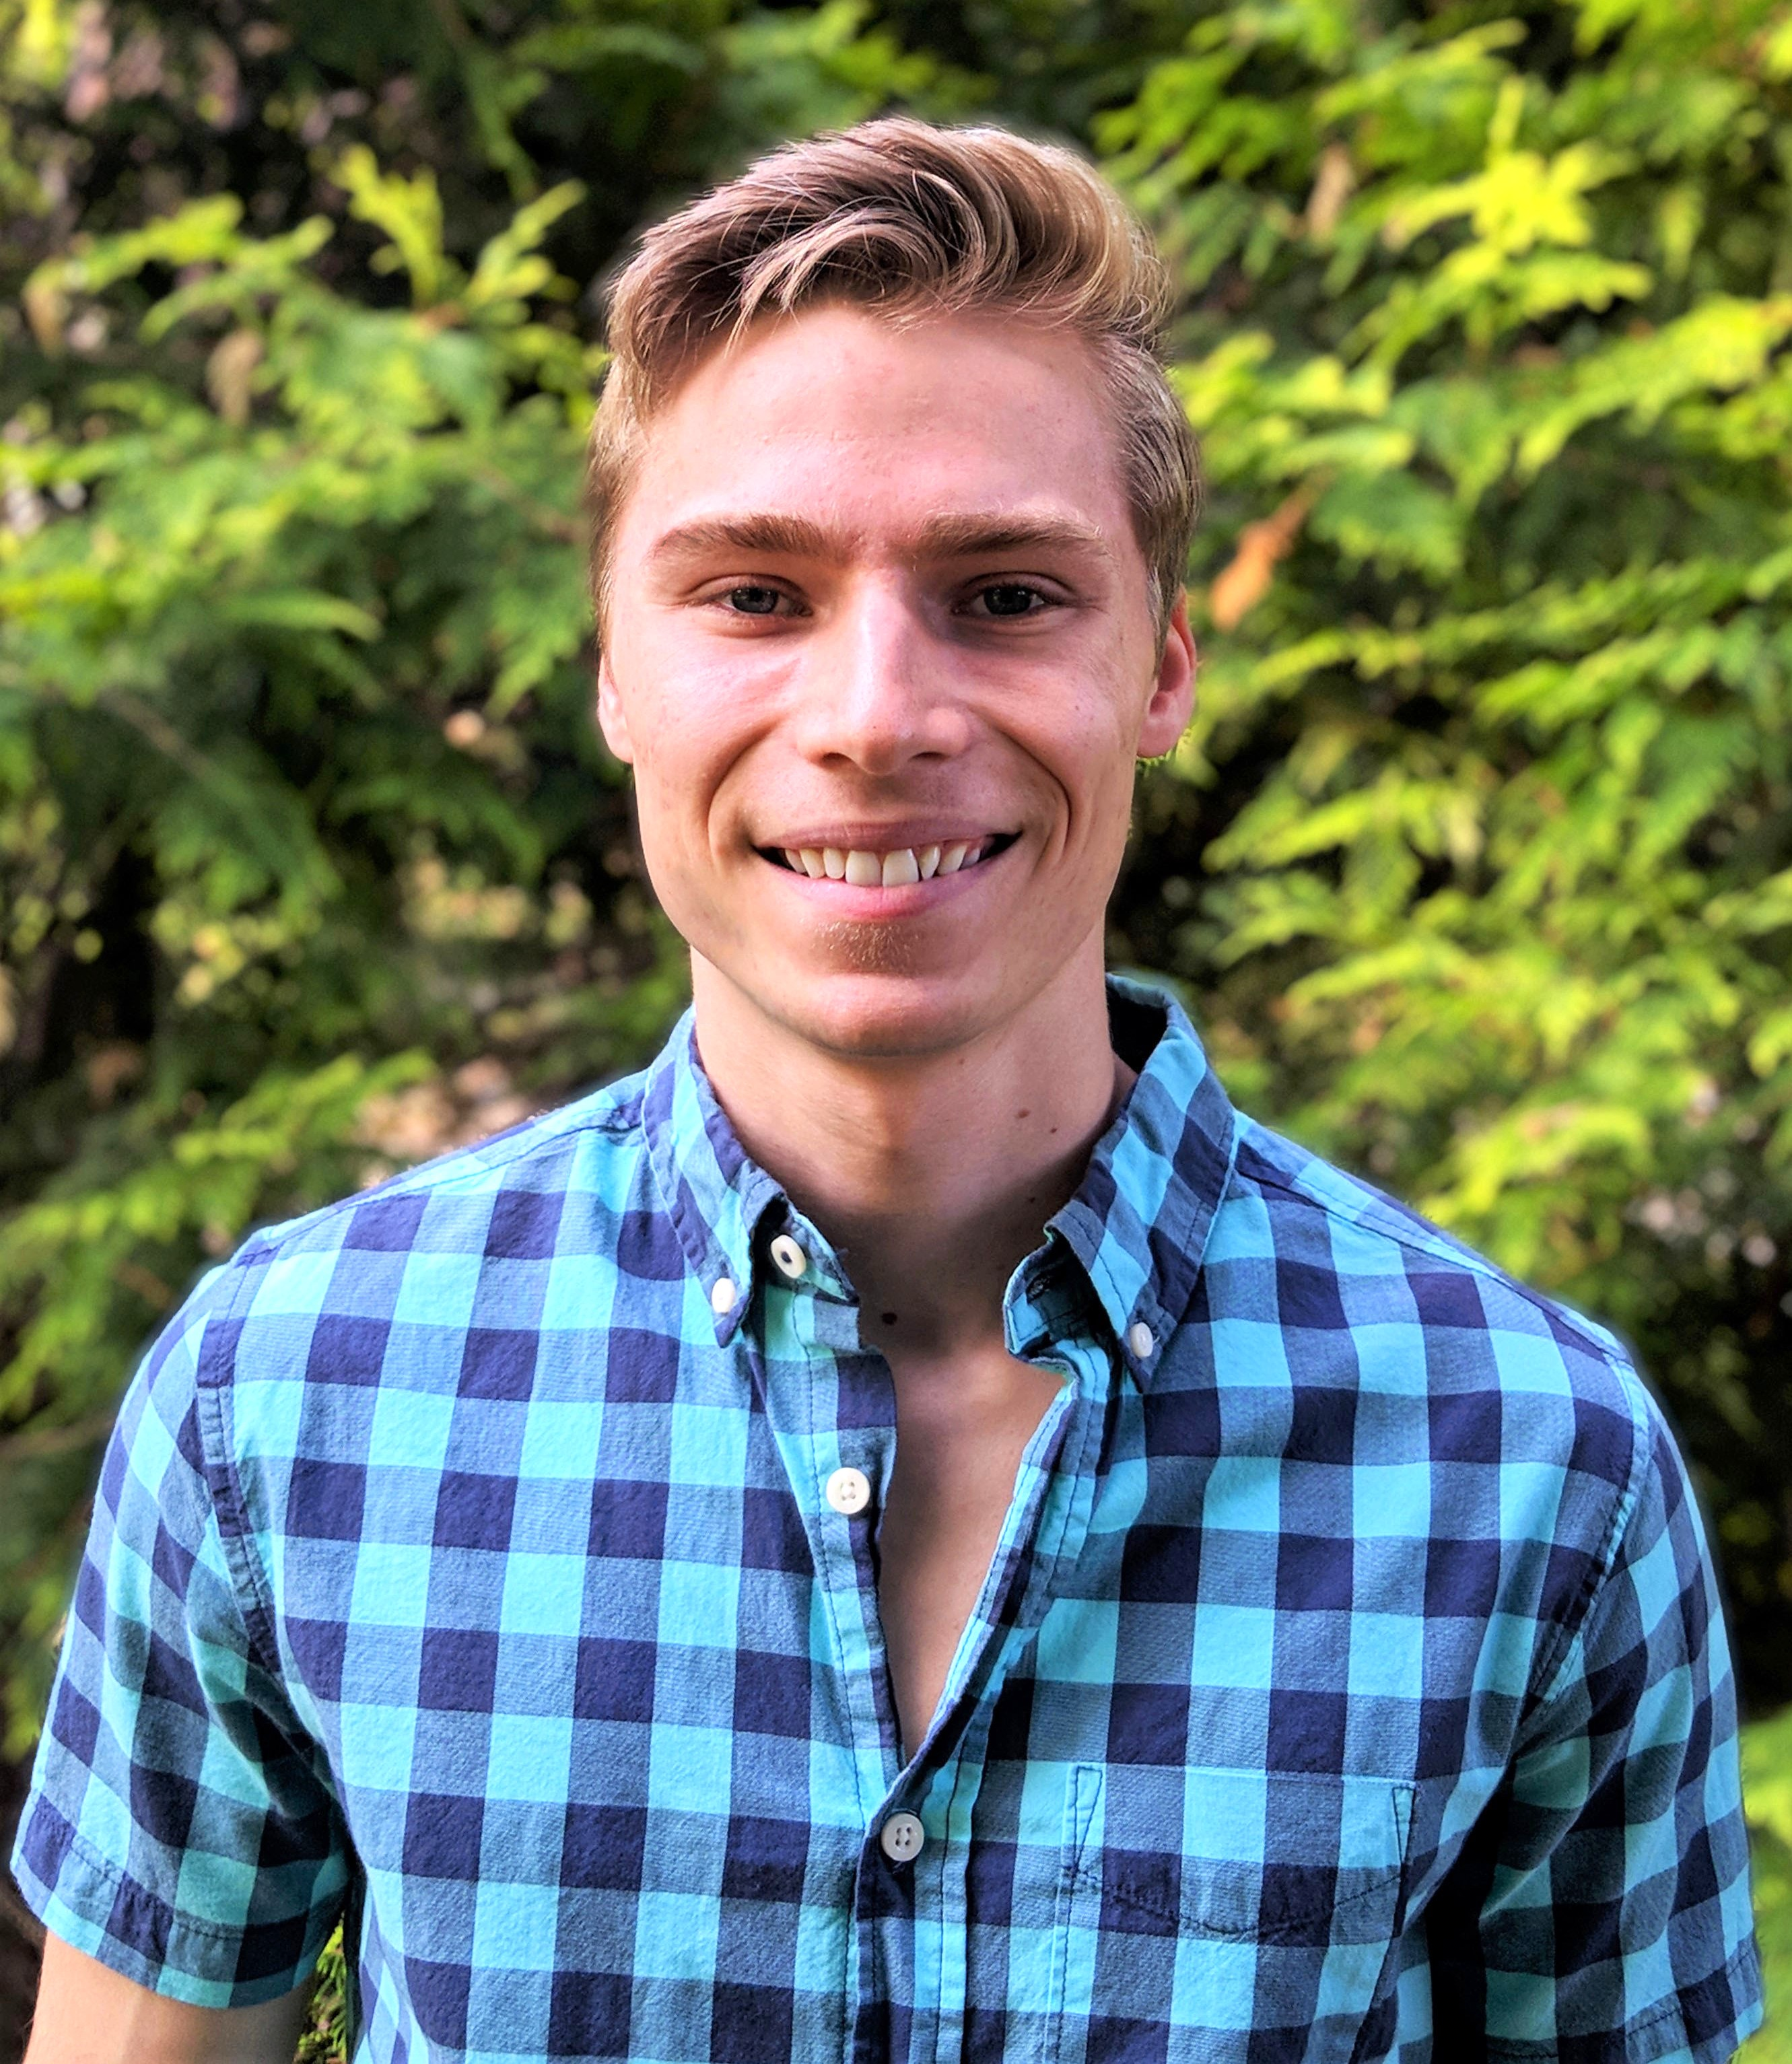
\includegraphics[width=3cm]{Jeremy_headshot_cropped.jpg}
	%	\vspace{-1cm}
	%\end{flushright}
	
	
	%----------------------------------------------------------------------------------------
	%	EDUCATION SECTION
	%----------------------------------------------------------------------------------------
	\vspace{-2em}
	\begin{rSection}{Education} 
		\begin{rSubsection}{Ludwig Maximilians Universit{\"a}t  M{\"u}nchen (LMU) \&\\Technische Universit{\"a}t M{\"u}nchen (TUM)}{\em Oct. 2019 -- Present}{}{}
			\vspace{-.5em}
			%			\item (In progress) MSci in Geophysics and Applied Physics (Joint Degree)
			\item (In progress) MSci in Geomaterials and Geochemistry
			\item Erasmus Mundus: Masters in Materials Science Exploring Large Scale Facilities
		\end{rSubsection}
		
		\begin{rSubsection}{Williams College}{\em 2015 -- 2019}{}{}
			\vspace{-.5em}
			\item B.A. in Physics with Honors, GPA 3.3
			\item Sigma Xi Inductee 
		\end{rSubsection}
		
%------------------------------------------------------------------------------------
%       Data Science Skills
%------------------------------------------------------------------------------------
	\begin{rSection}{Data Science Skills} \itemsep -2pt
	\begin{tabular}{ @{} >{}l @{\hspace{6ex}} l }
		Data Cleaning and Feature Engineering & SSH + VIM \\
		Command Line (BASH) & Probability and Statistics (Bayesian) \\
		Neural Networks and Deep Learning & Git and Version Control \\
		Natural Language Processing & Recommendation Systems		
	\end{tabular}
\end{rSection}
	
		
	\end{rSection}
	%----------------------------------------------------------------------------------------
	%	TECHNICAL STRENGTHS SECTION
	%----------------------------------------------------------------------------------------
	\newcommand{\CC}{C\nolinebreak\hspace{-.05em}\raisebox{.4ex}{\tiny\bf +}\nolinebreak\hspace{-.10em}\raisebox{.4ex}{\tiny\bf +}}
	\def\CC{{C\nolinebreak[4]\hspace{-.05em}\raisebox{.4ex}{\tiny\bf ++}}}
	
	\begin{rSection}{Technical Strengths}
		
		\begin{tabular}{ @{} >{\bfseries}l @{\hspace{6ex}} l }
			Programming Languages &  Python, MATLAB, SQL, JAVA, Arduino (C/\CC) \\
			Python Packages & Pandas, NumPy, sklearn, PyTorch, KERAS, TensorFlow, Seaborn \\
			Data Software & Mathematica, Quantum Espresso, Excel, LabView, LoggerPro \\
			Visualization Software & \LaTeX, Solid Works, VESTA, Adobe Illustrator, Adobe Photoshop   \\
		\end{tabular}
		
	\end{rSection}
	
	%----------------------------------------------------------------------------------------
	%	RESEARCH EXPERIENCE SECTION
	%----------------------------------------------------------------------------------------
	

	\begin{rSection}{Work Experience}
		\begin{rSubsection}{Amorphous Solids, Metallic Glasses, \& Metallurgy}{Summer 2019}{Postbac Researcher}{Yale University}
%			\vspace{-.5em}
%			\item[] {\em Advised by Jan Schroers, Professor of Physics}\hfill {\em Yale University}
			Nanomolded crystalline metals and analyzed the samples with SE and TE microscopy
		\end{rSubsection}
		
		
		\begin{rSubsection}{Soft Condensed Matter Physics}{2018 -- 2019}{Undergraduate Honors Thesis}{Williams College}
%			\vspace{-.5em}
%			\item[] {\em Advised by Katharine E. Jensen, Professor of Physics}\hfill {\em Williams College}
			Designed and built stretching apparatus for soft materials, collected data via confocal microsocopy, and analyzed data with MATLAB
		\end{rSubsection}
		%
		%----------------------------------------------------------------------------
		
		
		\begin{rSubsection}{Atomic, Molecular, and Optical Physics}{Summer 2017}{Undergraduate Research Assistant}{Williams College}
%			\vspace{-.5em}
%			\item[] {\em Advised by Protik K. Majumder, Professor of Physics}\hfill {\em Williams College}
			Programmed a PID controller, designed a deposition-rate detector for an indium cell chamber, and analyzed data with MATLAB and Mathematica
		\end{rSubsection}
		
	\end{rSection}
	
	
	
	
	
	
	%	EXAMPLE SECTION
	%----------------------------------------------------------------------------------------
	%
	%	\begin{rSection}{Achievements} \itemsep -2pt
	%		{Michigan Institute for Computational Discovery Fellow }\hfill {\em Spring 2015} \\
	%		{NSF GROW Fellowship Awardee}\hfill {\em Spring 2015} \\
	%		{Community Coordinated Modeling Center Research Winner} \hfill {\em Spring 2015} \\
	%		{NSF Graduate Research Fellowship Program Fellow}\hfill {\em Spring 2014}\\
	%		{Rackham Merit Fellow}\hfill {\em Fall 2013}\\
	%		{Template Developer for LaTeX} \hfill {\em September 2013 - Present} \\
	%		{Backpacker and Hiking Enthusiast - have climbed 7 $>$ 14,000 ft peaks}
	%	\end{rSection}
	
	
	
	
%	%------------------------------------------------------------------------------------
%	%       Publications
%	%------------------------------------------------------------------------------------
%	\begin{rSection}{Publications} \itemsep -2pt
%		\item {Toward and Adhesion Based Measurement of Strain-Dependent}\hfill {\em Undergraduate Thesis}\\ Surface Stress in Soft Solids
%	\end{rSection}
%	
	
	
	
	%------------------------------------------------------------------------------------
	%       Coursework
	%------------------------------------------------------------------------------------
	\begin{rSection}{Advanced Coursework} \itemsep -2pt
		\begin{tabular}{ @{} >{}l @{\hspace{6ex}} l }
			Multivariate Calculus & Linear Algebra \\
			Statistical Mechanics & Particle Physics \\ 
			Computational Materials Design & Partial Differential Equations \\
			Deep Learning & Machine Learning \\

			
		\end{tabular}
	\end{rSection}
	
		
	
	
	
	
\end{document}
